%!TeX root = SM_Thesis_Proposal.tex

\section{Introduction}
\label{sec:introduction}

Many containerization systems rely on Linux's isolation primitives, exposed via
the cgroups interface, in order to enforce the isolation between different
containers.\ cgroups allow for the control of many different resources,
including cpu, memory, and i/o. In this thesis we take a closer look at the way
the cpu isolation is used and enforced. 

\subsection{}

Kubernetes\cite{kubernetes}, for example, allows users to specify resource
requests and limits. Limits are directly passed on to the cgroups cpu.limit
interface. The way Linux in turn implements cpu limits is straightforward: the
underlying cgroups mechanism uses timers and careful accounting to ensure that
the processes that are running in the cgroup do not get more cpu time than they
are allowed to. 

Implementing the resource requests is more complicated, because in this
interface it is desirable that containers be allowed to burst when possible. For
example, a service $s_1$ might ask for 2 CPUs, but occasionally have bursts of
load. If it is on an otherwise empty machine with more than 2 CPUs, or
collocated with a different service that is experiencing less load than usual,
ideally $s_1$ would be able to use more than its allotted 2 CPUs. In order to
support this, Kubernetes relies on the cgroups' weight feature. Weights in
cgroups are implemented in a way that allows for the desired bursting: the cpu
time processes should get is determined by the ratio of the process's weight
($w_p$) to the weight of all \textit{runnable} processes ($W = \sum_i w_i$). For
example, suppose cgroup $cg_1$ is supposed to get 1 CPU and $cg_2$ 3 CPUs. The
ratio of their weights would be set to have a 1:3 ratio as well. That way, if
both cgroups have enough load to fill that capacity, then they are constantly in
contention for resources and the scheduler should ensure that $cg_1$ is running
$\frac{1}{3}$ of the time, and $cg_2$ $\frac{2}{3}$ of the time, amounting to
effectively $cg_1$ getting one CPU and $cg_2$ three, as desired. However, if
$cg_2$ happens to have less load, there will be times where it has no runnable
threads on some of the cores, and in those places the threads in $cg_1$ will
represent 100\% of the weight there and be able to get more cpu time.

\begin{figure*}[t]
    \centering
    \begin{subfigure}[t]{0.48\textwidth}
        \vspace{0pt}
        \centering
        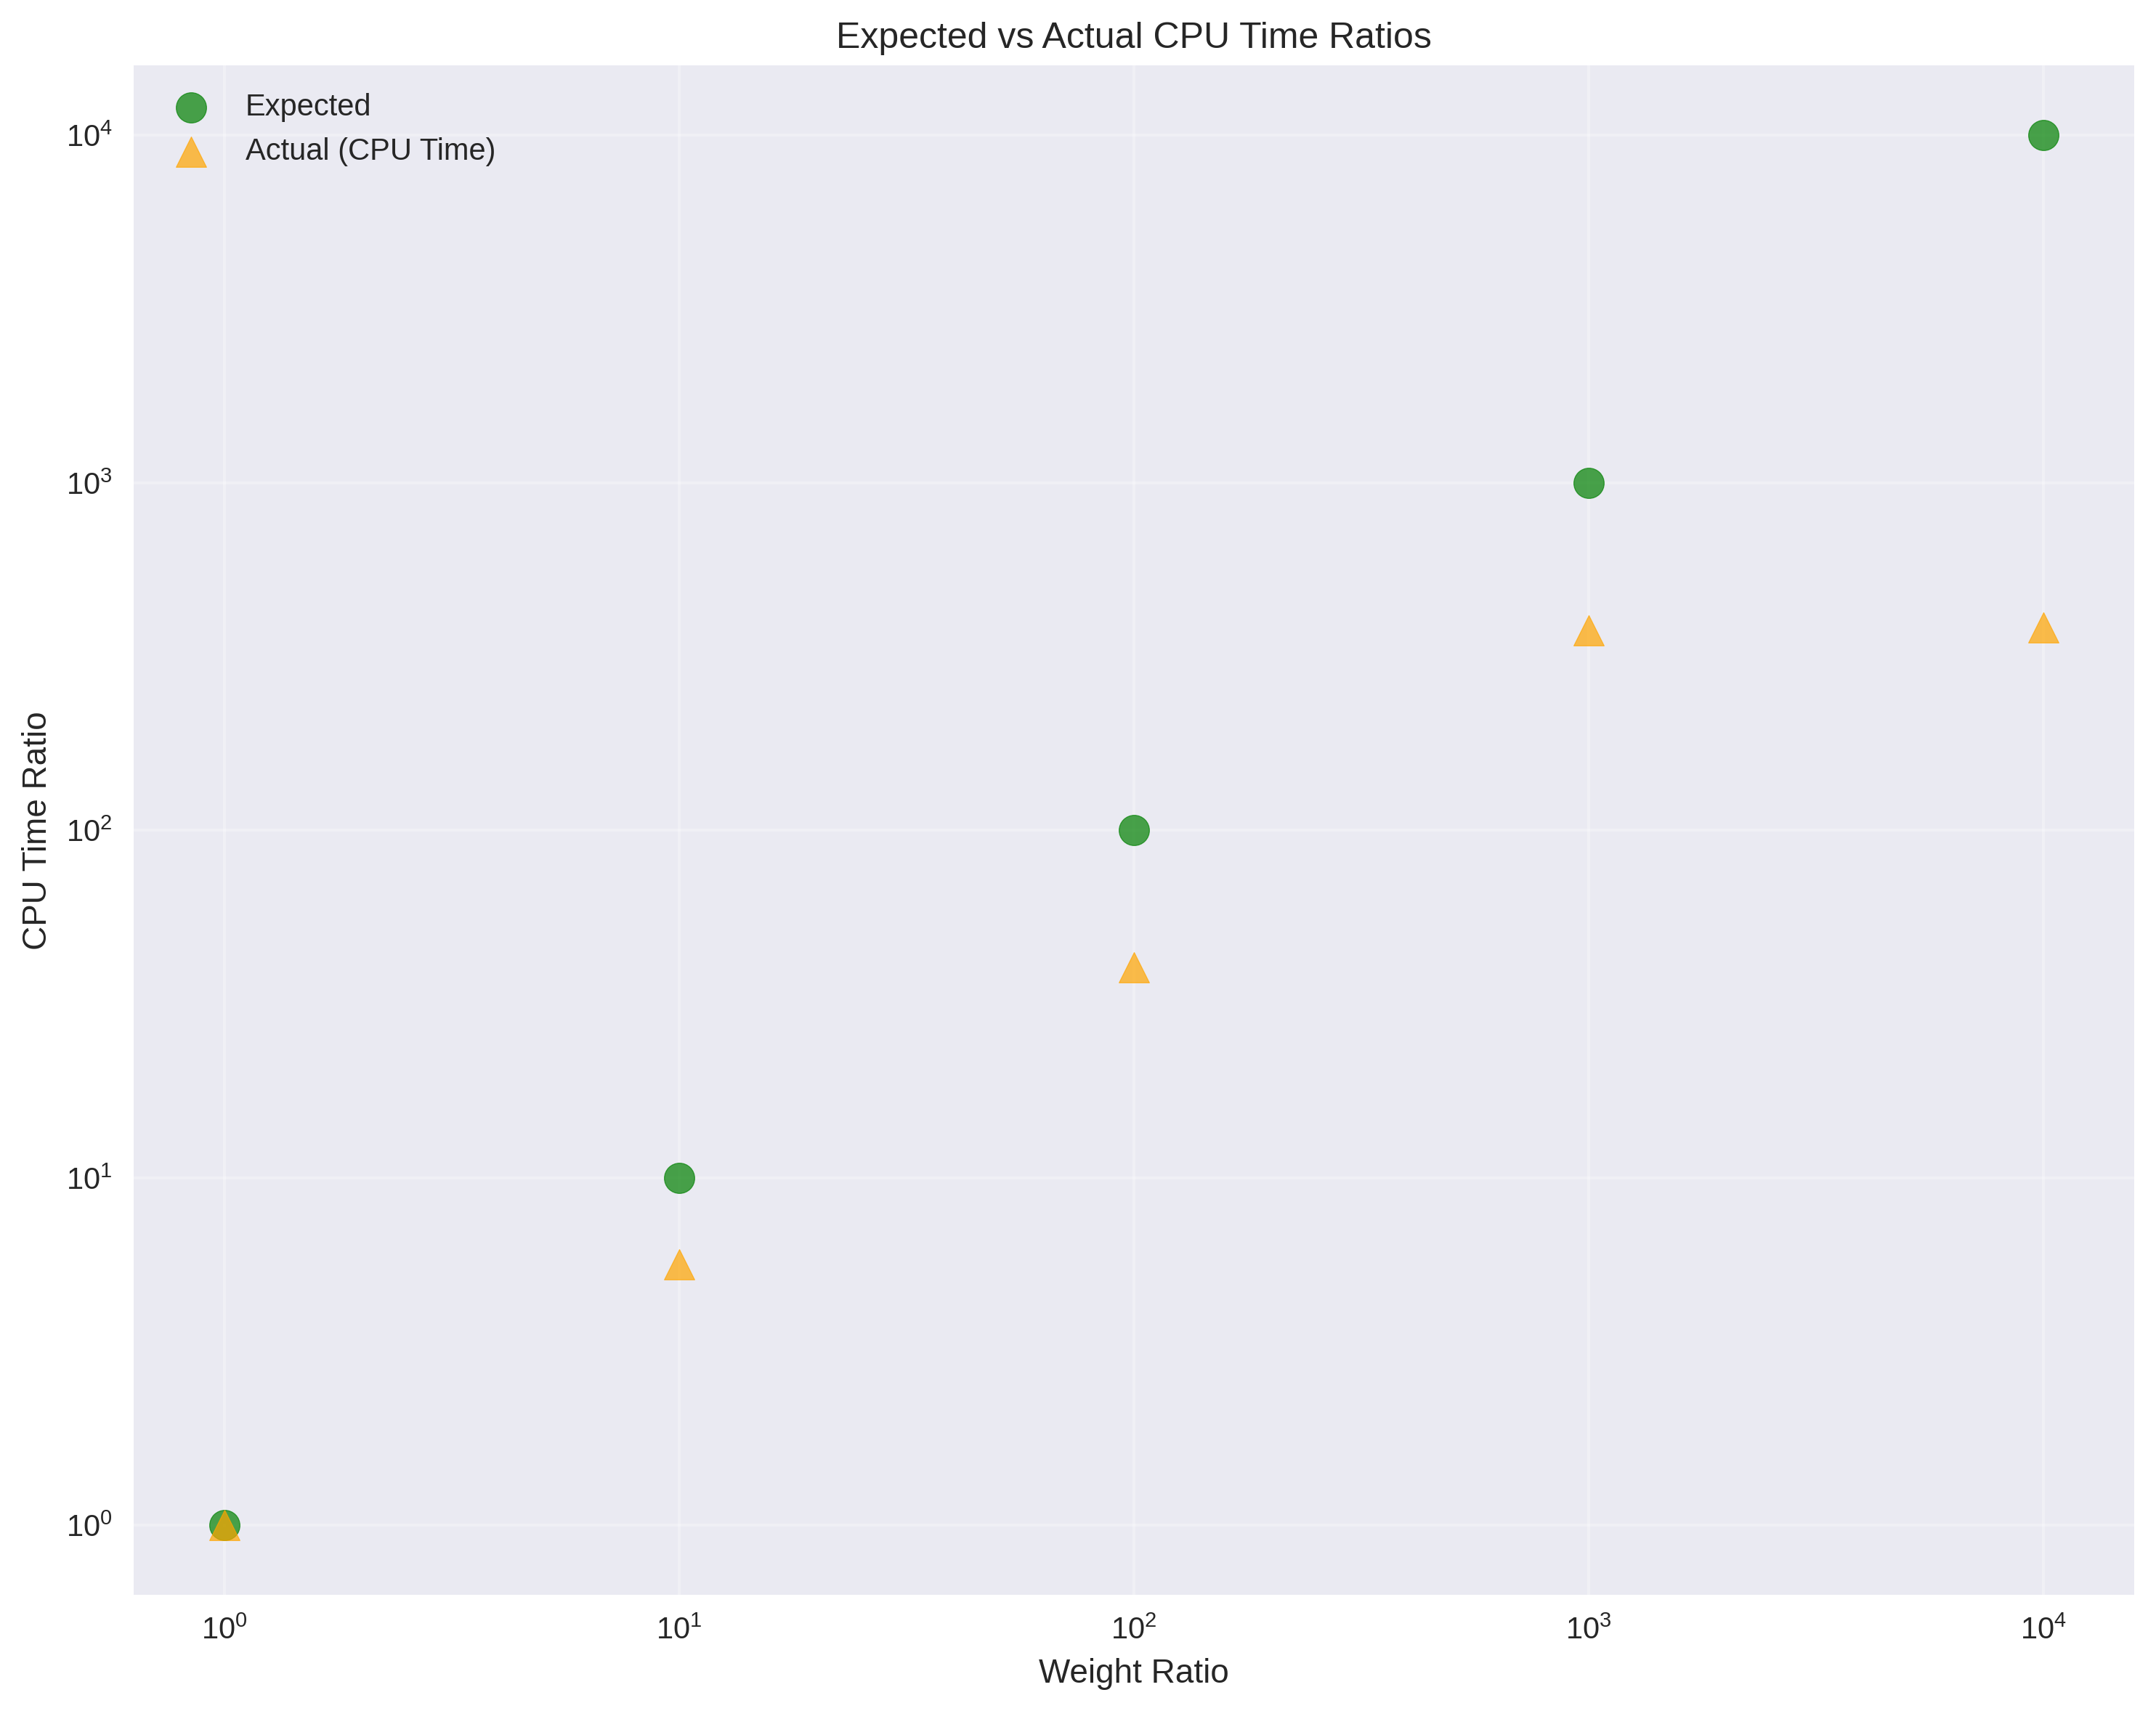
\includegraphics[width=\textwidth]{graphs/cpu-weight_split.png}
        \caption{The results of running two workloads across four cores with varying
        cpu.weight ratios, and measuring the actual CPU time they get.}\label{fig:cpu-weight_split}
    \end{subfigure}
    \hfill
    \begin{subfigure}[t]{0.48\textwidth}
        \vspace{12pt}
        \centering
        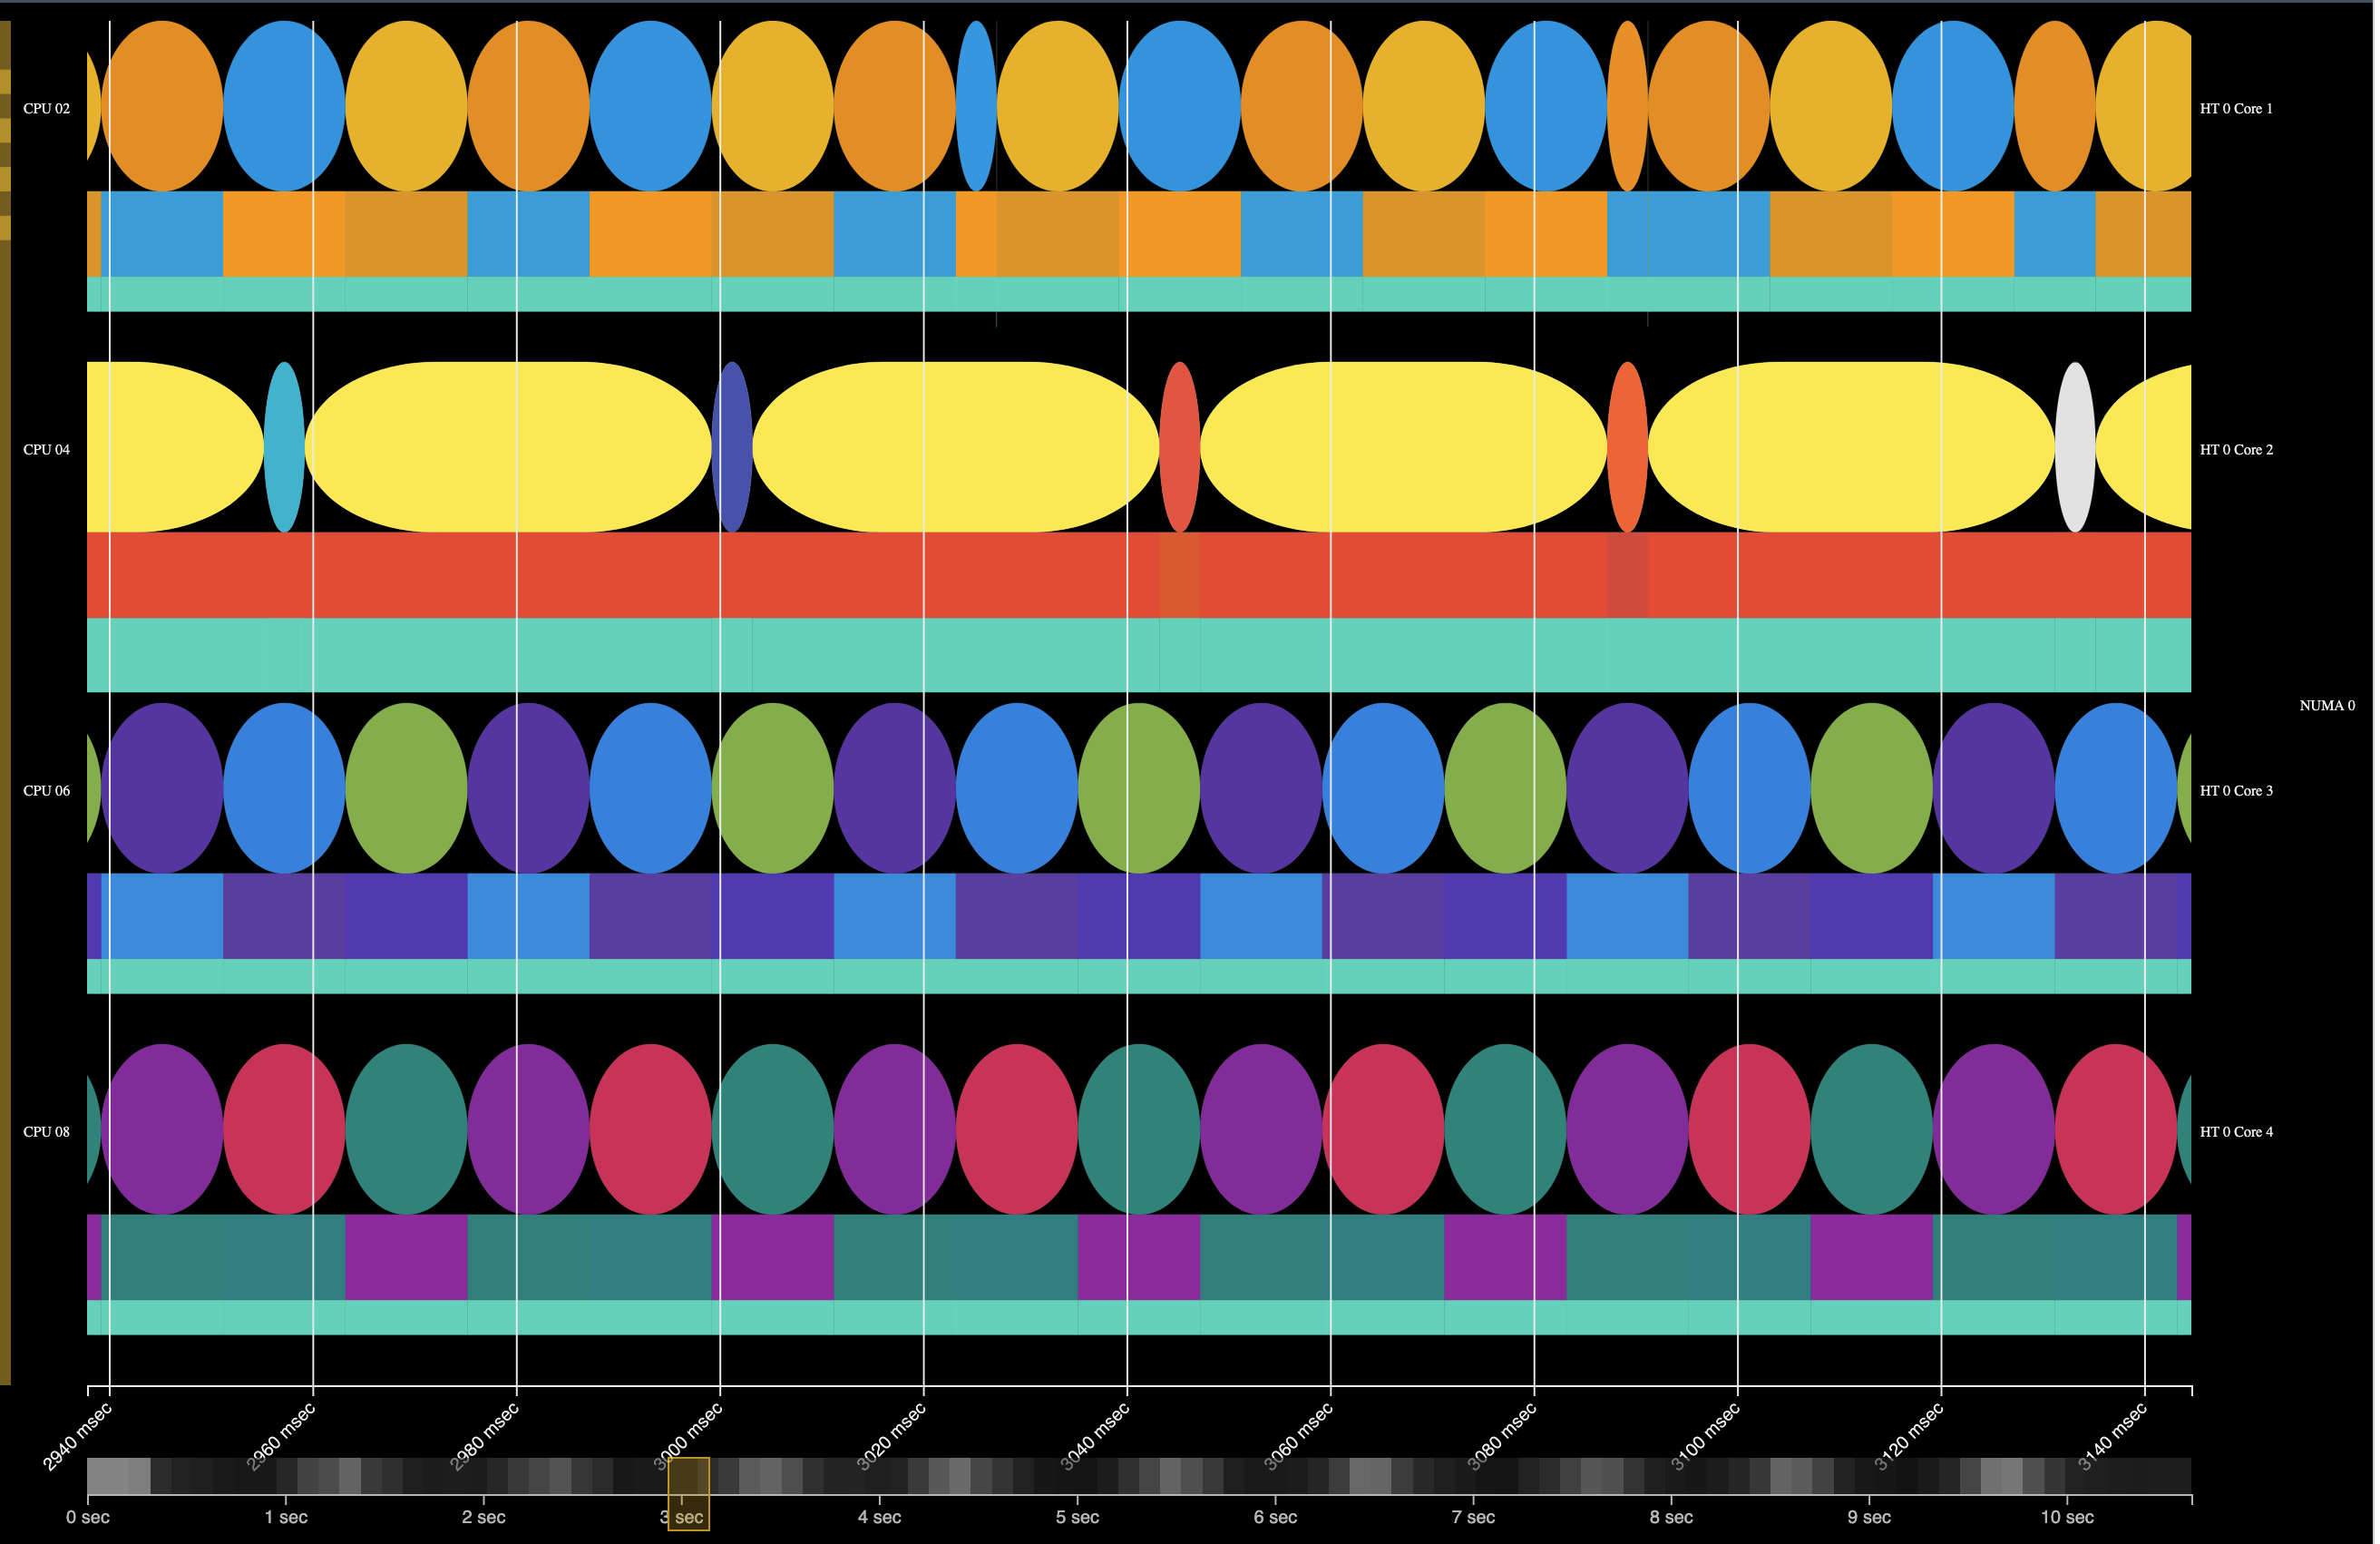
\includegraphics[width=\textwidth]{graphs/cpu-split-schedviz.png}
        \vspace{5.5pt}
        \caption{Each thread is a different color. Circles represent which
        thread is running on that core, while rectangles underneath show waiting
        but runnable threads.}\label{fig:schedviz-split}
    \end{subfigure}
    \caption{Comparison of CPU scheduling behavior using \texttt{cpu.weight} and actual thread activity visualized by SchedViz.}
\end{figure*}



The range of weights that the cgroup cpu.weight interface supports is [1,
10000]. However, a microbenchmark using 4 cpus shows that Linux is only
actually able to enforce a small fraction of the split ratios well. We run two
syntehtic cpu-bound workloads with ten threads each on four cores, with each
workload in its own cgroup. We vary the ratio of the cpu.weight of the cgroups,
and observe the cumulative cpu time that all the threads in each workload get.
We finally compare the expected cpu time ratio with the observed ratio. The
results are in Figure~\ref{fig:cpu-weight_split}. In order to understand the
reason for the discrepancy we visualize the scheduling decisions Linux is making
using schedviz\cite{schedviz} in Figure~\ref{fig:schedviz-split}, in this case
of the 100:1 split ratio. The main takeaway from this image is that, when two
threads of differing priorities are on the same core (as is true here for CPU
4), Linux does a great job of allocating the cpu time with the correct ratio.
However, for the other CPUs, the cpu time is being split equally betweent the
runnable threads, because they are in the same cgroup. As a result, on most of
the cores, the threads of different cgroups are not directly in contention with
each other. This leads to the lower weight cgroup getting more time than it
actually should.


\begin{figure*}[t]
    \centering
    \begin{subfigure}[t]{0.32\textwidth}
        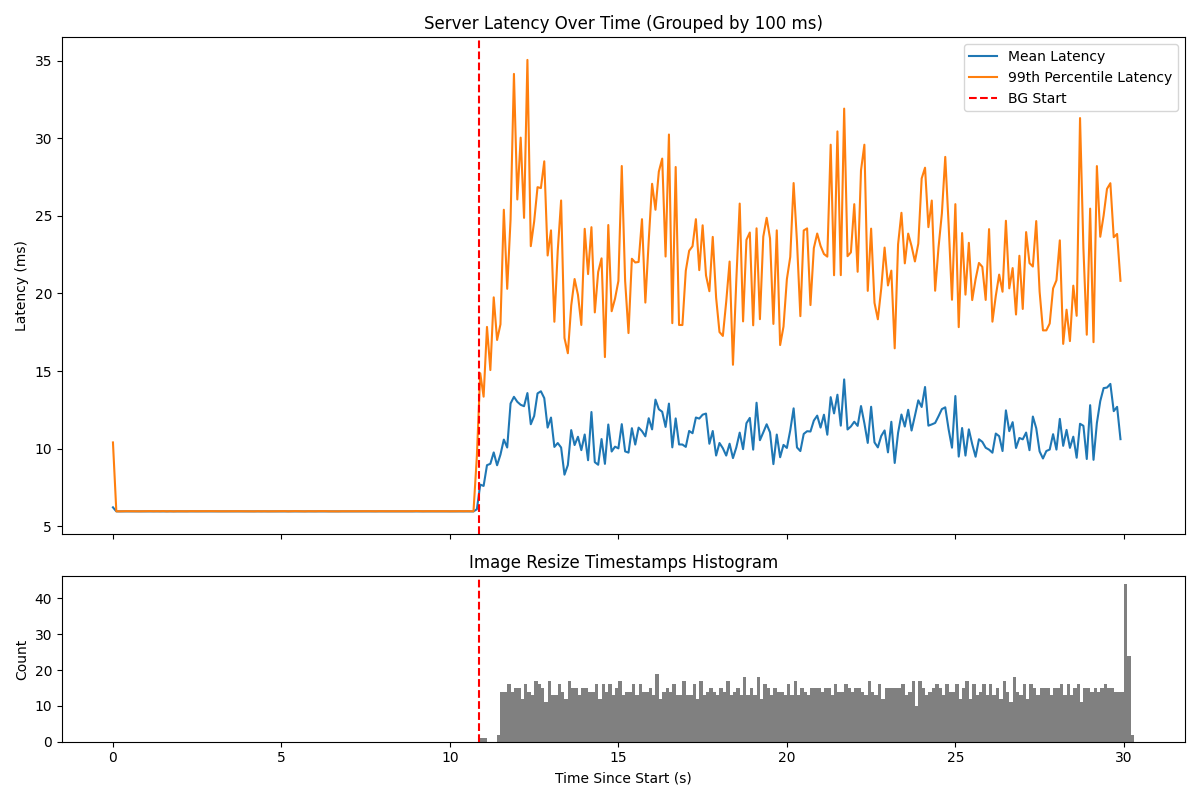
\includegraphics[width=\textwidth]{graphs/srv-lat-weight-low-two.png}
        \caption{Low load, two background tasks}\label{fig:srv-lat-weight-low-two}
    \end{subfigure}
    \hspace{\fill}
    \begin{subfigure}[t]{0.32\textwidth}
        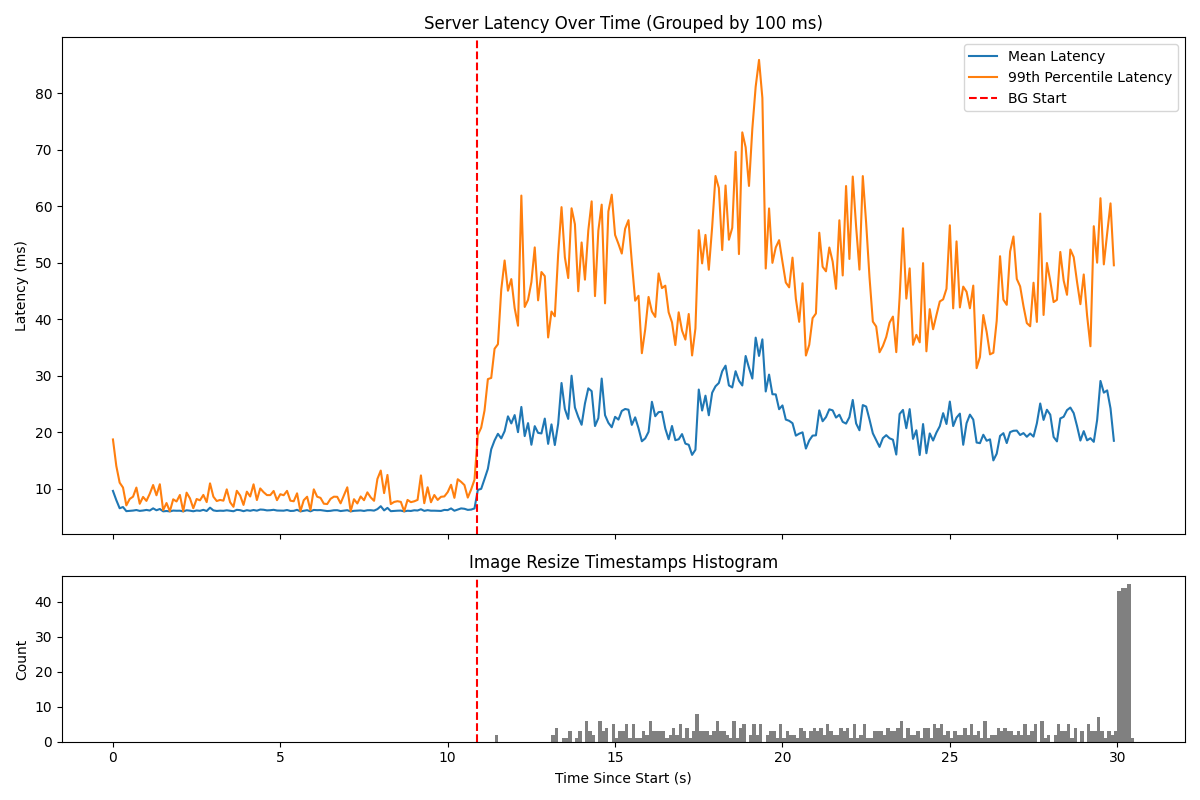
\includegraphics[width=\textwidth]{graphs/srv-lat-weight-high-two.png}
        \caption{High load; two background tasks}\label{fig:srv-lat-weight-high-two}
    \end{subfigure}
    \hspace{\fill}
    \begin{subfigure}[t]{0.32\textwidth}
        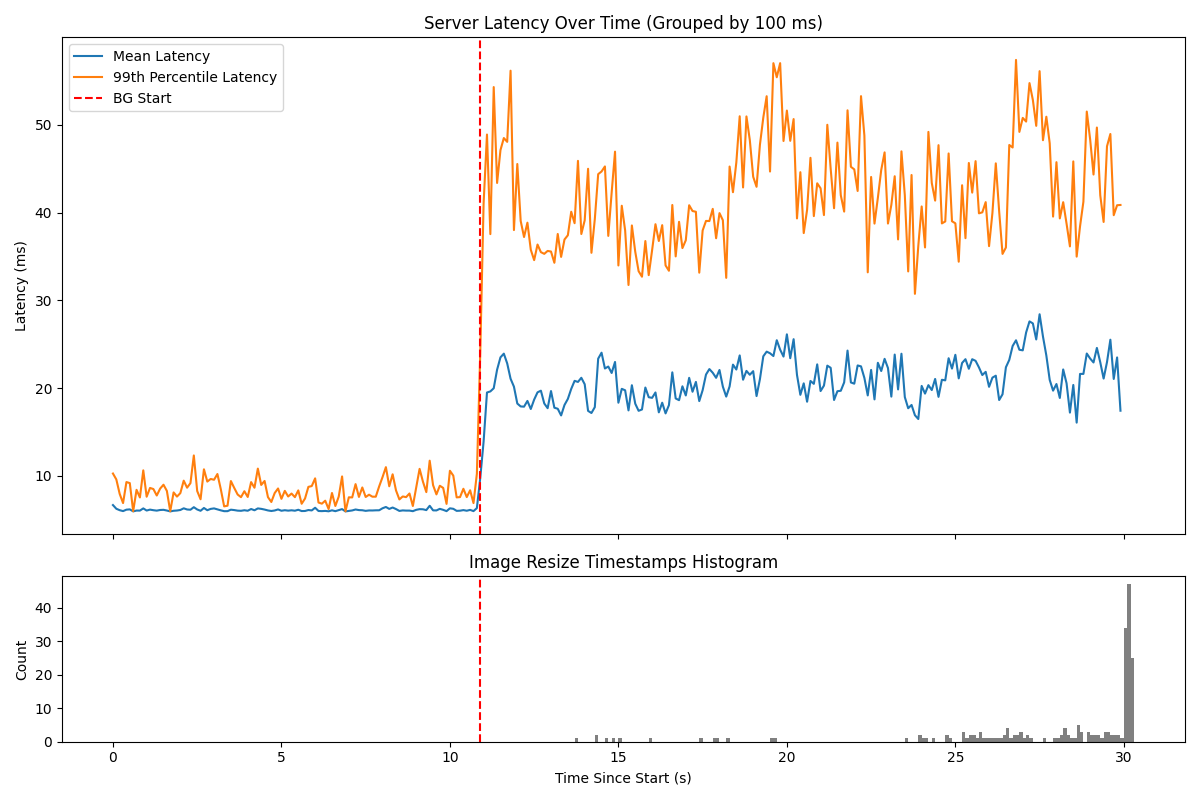
\includegraphics[width=\textwidth]{graphs/srv-lat-weight-high-sixteen.png}
        \caption{High load; sixteen background tasks}\label{fig:srv-lat-weight-high-sixteen}
    \end{subfigure}
    \caption{Latencies of the server and iteration counts of the background
    tasks in different load scenarios. Note the different y axis limits.}
\end{figure*}

In order to understand the practical implications of this inability of Linux to
enforce the cpu.weight split across multiple cores, we set up a more realistic
application. We run an LC server that processes requests coming in from an open
loop client, running on a separate machine. The client has 100 connections to
the server, each connection creates a separate server thread that reads from the
socket and synchronously processes requests in a tight loop. The server threads
run in a cgroup with the highest possible weight: 10000. The server initially
runs on an uncontended four cores, during which time the cpu utilization of the
server is around 83\%. After $\sim$10 seconds, we start two background tasks
on the same four cores, each performing an image resize job. Each background
task is in its own cgroup, which both have the lowest possible weight, 1. We
then measure the latencies experienced by the LC server, before and after
starting the background tasks; Figure~\ref{fig:srv-lat-weight-low-two} shows the
results. We see that mean latencies spike up from steady at just under 6ms to as
high as 13ms, and much higher for 99th percentile latencies.

With higher baseline load for the LC server the spikes get worse, in
Figure~\ref{fig:srv-lat-weight-high-two} the utilization of the uncontended server load is around 96\%
(with the same two BE tasks). Although, interestingly, with more background
tasks, the latency degradation doesn't get proportionally worse:
Figure~\ref{fig:srv-lat-weight-high-sixteen} shows the experiment with the same load as
Figure~\ref{fig:srv-lat-weight-low-two}, but with 16 background tasks instead of 2. That
makes sense, given what we have seen the explanation is: the problem is that LC
threads are not even queued on some cores, not that they don't get the share
they deserve.







